\section{总体介绍}

\begin{frame}
    \frametitle{开发情况}

    \begin{itemize}
        \item 内核一共 1.6 万行代码
        \item 实现了 77 条系统调用,能够支持决赛第一阶段除网络外的测试
        \item \strong{同一份二进制可同时在多个平台 (QEMU / VisionFive V2) 上启动}
        \item \strong{能够在模拟器上运行 Linux}
    \end{itemize}

\end{frame}

\begin{frame}
    \frametitle{总体架构}
    \begin{figure}
        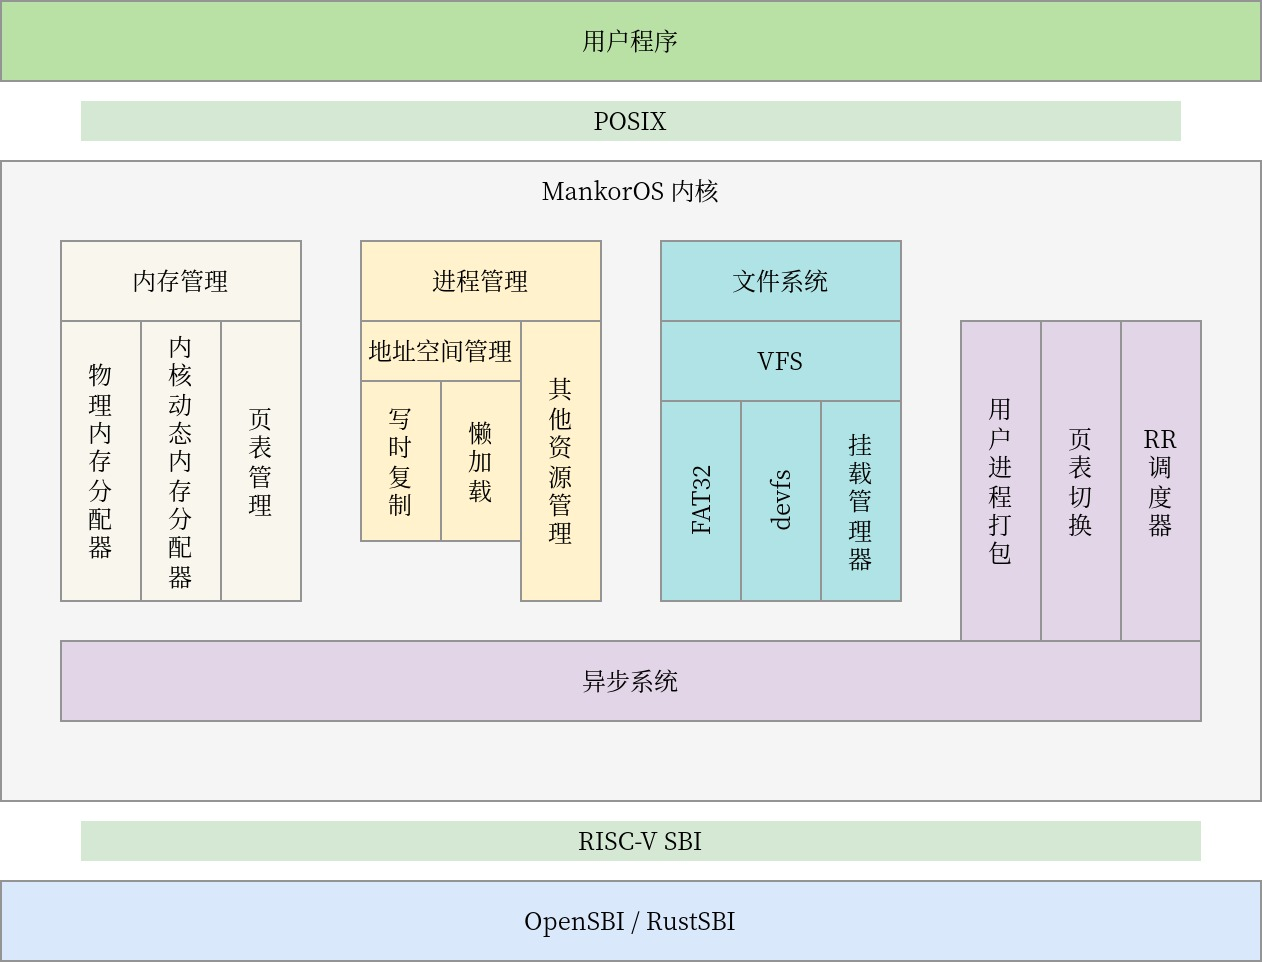
\includegraphics[width=.6\textwidth]{assets/Arch.jpg}
    \end{figure}

\end{frame}

\begin{frame}
    \frametitle{在线测试成绩}
    \begin{figure}
        \centering
        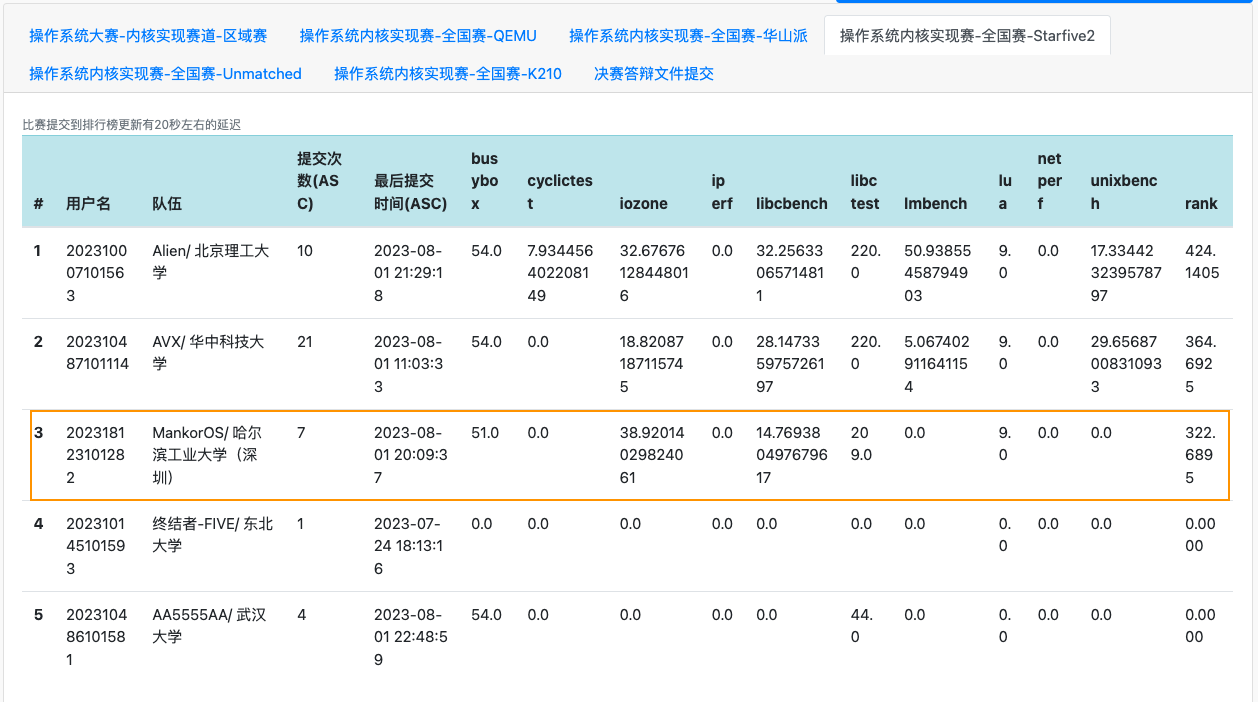
\includegraphics[width=.7\textwidth]{assets/rank.png}
    \end{figure}

\end{frame}

\begin{frame}
    \frametitle{开发宗旨}

    \vfill
    \begin{center}
        \begin{LARGE}
            \strong{做往年参赛队伍没有做过的功能}
        \end{LARGE}

        \hspace*{\fill}

        当然,必须是有用的功能
    \end{center}
    \vfill
\end{frame}